\documentclass[conference]{IEEEtran}
\IEEEoverridecommandlockouts
% The preceding line is only needed to identify funding in the first footnote. If that is unneeded, please comment it out.
\usepackage{cite}
\usepackage{amsmath,amssymb,amsfonts}
\usepackage{algorithmic}
\usepackage{graphicx}
\usepackage{textcomp}
\usepackage{xcolor}
\usepackage{multirow}
\def\BibTeX{{\rm B\kern-.05em{\sc i\kern-.025em b}\kern-.08em
    T\kern-.1667em\lower.7ex\hbox{E}\kern-.125emX}}
\begin{document}

\title{Speaker Recognition in the Wild\\}

\author{\IEEEauthorblockN{Gabriele Cerizza}
\IEEEauthorblockA{\textit{Department of Computer Science} \\
\textit{University of Milan}\\
Milan, Italy \\
gabriele.cerizza@studenti.unimi.it}
}

\maketitle

\begin{abstract}
Speaker recognition is the task of recognizing a person from their utterances, either to classify or to verify the identity of a given speaker. In this work, we review the main techniques developed to tackle speaker recognition and compare the performance of different neural network models on this task, using a dataset collected under real-world conditions.  
\end{abstract}

\begin{IEEEkeywords}
speaker recognition, speaker identification, speaker verification, convolutional neural networks, attention
\end{IEEEkeywords}

\section{Introduction}

Speaker recognition is a challenging task that includes two problems: speaker identification and speaker verification~\cite{kabir2021survey,hajibabaei2018unified,chung2020defence}. 

Speaker identification is a closed-set problem akin to classification, in which the model has to identify the person to whom a given utterance belongs. The model is trained on utterances from each speaker. Speaker verification aims at validating whether a given utterance belongs to a given person. In academic research, this is treated as an open-set problem in which the model has to determine if two utterances belong to the same person. During evaluation, the model is presented with pairs of utterances belonging to speakers not included in the training set.

% Speaker recognition can be further categorized as text-dependent or text-independent, in relation to the fact that the content of the utterances is fixed or not.

Speaker recognition applications encompass security control, online banking, retrieval, forensic tools and human computer interaction systems. A speaker recognition model can be also employed as part of a speaker diarization pipeline \cite{chung2018voxceleb2}.

In our research we compared the performance of different neural network models, which allowed us to tackle both speaker identification and verification at the same time. To train and evaluate the models, we used data collected ``in the wild'', i.e. under real-world conditions.

% To train and evaluate the models, we used data from VoxCeleb1~\cite{nagrani2020voxceleb}. These data were collected ``in the wild'', that is under real-world conditions where speech segments may be affected by the environment, like background noise and cross-talk.

The remainder of the report is organized as follows. In Section~\ref{sec:related_works} we discuss related works in the field of speaker recognition. In Section~\ref{sec:dataset} we illustrate the characteristics of the dataset and the features. In Section~\ref{sec:models} we describe three neural networks, whose performances are compared and discussed in Section~\ref{sec:results}. Finally, Section~\ref{sec:conclusions} contains our concluding remarks.  


\section{Related works}
\label{sec:related_works}

\subsection{Model Architectures}

%In particular, the interest in the field has grown in recent years, owing to the availability of large-scale datasets and to the increased computational power afforded by GPUs, which allows us to train deep neural networks.

Speaker recognition methods have been widely studied in literature and, over the years, a particular approach became predominant. The idea is to produce fixed-sized feature representations of speech segments, which can then be processed by a classifier or directly compared. With the advent of neural networks, these speaker representations, known as ``embeddings'', were obtained as the output of a bottleneck layer trained for classification. Embeddings proved to be robust with respect to acoustic conditions and discriminative with respect to speakers, thus yielding accurate results. 

% Examples of such neural embeddings include d-vectors~\cite{variani2014dvectors} and, more recently, x-vectors~\cite{snyder2017deep,snyder2018xvectors}.

To perform speaker recognition with neural networks, an architecture composed of three blocks is traditionally employed~\cite{okabe2018asp}. The first block, also called ``trunk'', receives as input acoustic features such as MFCCs or Mel spectrograms and produces frame-level features. Typical layers of this block include CNNs, Time-Delay Neural Networks (TDNN)~\cite{peddinti2015timedelay}, mostly implemented as dilated convolution, and Recurrent Neural Networks such as Long Short-Term Memory (LSTM) networks. 

% Popular architectures for the first block are borrowed from the image recognition domain, such as ResNet~\cite{he2016resnet}, VGG~\cite{simonyan2014vgg} and, recently, Visual Transformers like CoAtNet~\cite{dai2021coatnet}. 

The second block is required to aggregate the frame-level features, which have varying length depending on the length of the speech segment, into fixed dimensional utterance-level features. This block usually consists of a fully connected layer stacked on top of a pooling layer. Many different pooling layers have been developed: from simply taking the average over the temporal dimension to sophisticated attention mechanisms~\cite{cai2018exploring}. The output of this block is the aforementioned embedding.

Finally, the third block contains the loss function, possibly preceded by a fully connected layer projecting the embedding into a dimension whose size is equal to the number of speakers. 

% Since the network is usually trained for multi-class classification, the loss function mixes and matches a plethora of Softmax variants with Cross-entropy loss.

% It is worth to note that models, especially in competitions like the VoxCeleb Speaker Recognition Challenge\footnote{https://www.robots.ox.ac.uk/$\sim$vgg/data/voxceleb/competition2021.html}, are often combined using fusion or ensemble techniques.

\subsection{Speaker Verification Peculiarities}

\paragraph{Scoring}After training the models for classification, a further step is necessary to compare utterances. During evaluation, embeddings are extracted for each utterance and then compared pairwise. These comparisons may be carried out with backend systems like Probabilistic Linear Discriminant Analysis (PLDA), possibly trained on a different dataset ~\cite{snyder2017deep}. However, more recently, embeddings have been compared simply by cosine similarity, achieving gains in performance~\cite{cai2018exploring}.

\paragraph{Score normalization}To produce well calibrated and reliable scores, normalization is often applied. A popular score normalization technique is ``Adaptive S-Norm'' (AS-Norm)~\cite{matejka2017asnorm}.

Let $s(\cdot,\cdot)$ be the score between two embeddings, $\mathcal{E}^{\text{top}}_e$ be the cohort of the $N$ closest embeddings to the enrollment utterance $e$ and $\mathcal{E}^{\text{top}}_t$ be the cohort of the $N$ closest embeddings to the test utterance $t$. Furthermore, let 
\begin{equation}
    S_e(\mathcal{E}^{\text{top}}_e) = \{(s,\varepsilon)\}_{\forall\varepsilon \in \mathcal{E}^{\text{top}}_e}~,
    S_e(\mathcal{E}^{\text{top}}_t) = \{(s,\varepsilon)\}_{\forall\varepsilon \in \mathcal{E}^{\text{top}}_t}~. 
\end{equation}
The normalized score is computed as
\begin{multline}
    s(e,t) = \frac{1}{2} \cdot \Bigg(\frac{s(e,t) - \mu(S_e(\mathcal{E}^{\text{top}}_e))}{\sigma(S_e(\mathcal{E}^{\text{top}}_e))} + \\
    \frac{s(e,t) - \mu(S_e(\mathcal{E}^{\text{top}}_t))}{\sigma(S_e(\mathcal{E}^{\text{top}}_t))}\Bigg)
    ~.
\end{multline}

\paragraph{Metrics}Once the similarity score between each pair of embeddings has been computed, we need to evaluate how good the model is in deciding whether the speech segments belong to the same speaker. To this end, various metrics have been proposed. Two notable metrics are Equal Error Rate (EER) and Minimum Detection Cost Function (MinDCF)~\cite{brummer2013bosaris,nist2018}. 

EER is defined as the point on the Receiver Operating Characteristic (ROC) curve in which $P_{\text{miss}} = P_{\text{fa}}$, where $P_{\text{miss}}$ is the ratio of samples belonging to the same speaker classified as dissimilar and $P_{\text{fa}}$ is the ratio of dissimilar samples classified as belonging to the same speaker. EER can be considered as a summary of the ROC curve.

On the other hand, MinDCF is derived from the normalization of the following weighted sum of misses and false-alarm error probabilities for a given decision threshold $\theta$:
\begin{equation}
    C_{\text{miss}} \times P_{\text{target}} \times P_{\text{miss}}(\theta) +
    C_{\text{fa}} \times (1 - P_{\text{target}}) \times P_{\text{fa}}(\theta) ,
\end{equation}
where $C_{\text{miss}}$ and $C_{\text{fa}}$ are respectively the cost of misses and false-alarms and $P_{\text{target}}$ is the \textit{a priori} probability of the specific speaker. The costs are usually fixed to 1. We refer to~\cite{nist2018} for the mathematical details of the normalization operation.

% \paragraph{Pairwise Losses}Another difference between speaker identification and recognition lies in the choice of loss functions. Some models employ pairwise losses such as Triplet loss or Contrastive loss~\cite{cai2018exploring,chung2019delving}. The drawback of these losses is that they are notoriously difficult to train with and require careful fine-tuning~\cite{nagrani2020voxceleb}. Most state-of-the-art models now adopt Softmax variants, discussed below.

\subsection{Pooling Layers}

\paragraph{Temporal Average Pooling (TAP)}This is the simplest pooling, which takes the mean of the features along the time domain~\cite{cai2018exploring,chung2019delving}. In this way, all frames equally contribute to the utterance representation.

\paragraph{Self-Attentive Pooling (SAP)}Under the assumption that not all frames are equally informative, SAP uses an attention mechanism to learn which weight to assign to each frame. The frames are then multiplied by their respective weights and summed to obtain the utterance-level representation~\cite{cai2018exploring}. A SAP layer can act as a Voice Activity Detection (VAD) layer~\cite{desplanques2020ecapa}.

More formally, let $W$, $b$ and $\mu$ be learnable parameters. Additionally, let $\{x_1,\dots,x_T\}$ be the time domain features of a given utterance. We first compute the attention weights $w_t$ as
\begin{equation}
    h_t = \text{tanh}(Wx_t + b)~,
\end{equation}
\begin{equation}
    w_t = \frac{\text{exp}(h_t^T\mu)}{\sum_{t=1}^T\text{exp}(h_t^T\mu)}~.
\end{equation}
Finally, we take the sum
\begin{equation}
    e = \sum_{t=1}^Tw_tx_t~.
\end{equation}

\paragraph{Other}Other notable pooling layers have been proposed. One of them is Self Multi-Head Attention Pooling, which splits the input to the layer into $N$ sequences, applies SAP to each of them and then concatenates the results~\cite{india2019selfmha}. Another one is Attentive Statistics Pooling (ASP), which combines SAP with mean and standard deviation statistics~\cite{okabe2018asp}.

\subsection{Softmax for Speaker Recognition}

Neural networks for speaker recognition may be effectively trained with Softmax and Cross-entropy loss, which are traditionally employed for classification problems. 

The \textit{caveat} is that Softmax penalizes only classification errors, without enforcing intra-class compactness and inter-class separation~\cite{chung2020defence}. This makes Softmax unsuited to learn discriminative features, which map utterances belonging to the same speaker close to each other and far from utterances belonging to other speakers~\cite{liu2019large}. To remedy this, angular based losses have been developed.

% originally in the context of face recognition, and have now become widespread in the speaker recognition field, reportedly achieving an improved performance.

This class of loss functions is chiefly represented by Angular Additive Margin Softmax (AAM Softmax or ArcFace)~\cite{deng2019arcface}. This function introduces an angular margin penalty $m$, which forces the cosine similarity between the sample and its true class to be $m$ more than the cosine similarity between the sample and wrong classes. This difference is also multiplied by a scale factor $s$, which prevents the gradient from getting too small~\cite{chung2020defence,hajibabaei2018unified}. On the downside, it is difficult to train with AAM Softmax and results are sensitive to the parameter values.

Recently, Sub-center AAM Softmax (SC AAM Softmax) has been proposed~\cite{deng2020subarcface}. This loss function relaxes the intra-class compactness constraint by incorporating $K$ sub-centers for each class and forcing each sample to be close to any of the positive sub-centers. It is expected that one dominant sub-center will contain the majority of ``clean'' samples belonging to the class, while the hard and noisy samples will gravitate toward the non-dominant sub-centers. As such, SC AAM Softmax is more robust to noise.

\section{Data and Features}
\label{sec:dataset}

\subsection{Dataset}

For our study, we elected to use the VoxCeleb1 dataset, which is characterized by speech segments collected ``in the wild'' from YouTube~\cite{nagrani2020voxceleb,chung2018voxceleb2,chung2019delving}. This dataset is particularly challenging due to the fact that the samples present both extrinsic and intrinsic variations. Extrinsic variations include background noise, chatter, music, laughter, cross-talk and varying room acoustics. Intrinsic variations concern the heterogeneity of age, gender and nationality of the speakers. 

The VoxCeleb1 dataset consists of over 150,000 utterances from 1,251 celebrities. However, due to hardware constraints, we were forced to confine our experiments to a randomly sampled subset. We extracted all the utterances of 100 randomly chosen speakers, while retaining the gender proportions to guarantee the representativeness of the sample. We kept the official splits for the training, validation and test sets that were provided for identification. To evaluate the verification capabilities of the models, we used utterances from 10 further speakers not present in the subset previously described. Some statistics on both the dataset and the subsets are provided in Table~\ref{tab:dataset}.

\begin{table}[htbp]
    \caption{VoxCeleb1 Dataset Statistics}
    \begin{center}
        \begin{tabular}{|c|c|c|c|c|}
        \cline{3-5}
        \multicolumn{2}{c|}{\textbf{}} & \textbf{Full Dataset} & \textbf{Identif. Set} & \textbf{Verif. Set}\\
        \hline
        \multicolumn{2}{|c|}{\textbf{Speakers No.}} & 1,251 & 100 & 10\\
        \hline
        \multicolumn{2}{|c|}{\textbf{Samples No.}} & 153,516 & 13,042 & 758 \\
        \hline
        \multirow{2}{*}{\textbf{Gender}} & \textit{Male} & 0.55 & 0.55 & 0.50 \\
        & \textit{Female} & 0.45 & 0.45 & 0.50 \\
        \hline
        \multirow{4}{*}{\textbf{Nationality}$^{\mathrm{a}}$} & \textit{USA} & 0.64 & 0.59 & 0.80 \\
        & \textit{UK} & 0.17 & 0.19 & 0.10 \\
        & \textit{Canada} & 0.04 & 0.02 & - \\
        & \textit{Australia} & 0.03 & 0.04 & - \\
        \hline
        \multirow{2}{*}{\textbf{Seconds}} & \textit{Mean} & 8.25 & 8.20 & 8.05 \\
        & \textit{Std} & 5.31 & 5.35 & 5.14 \\
        \hline
        \multicolumn{5}{l}{$^{\mathrm{a}}$Only the four most frequent nationalities in the entire dataset are listed.}
        \end{tabular}
        \label{tab:dataset}
    \end{center}
\end{table}

\subsection{Features}

As input features, we extracted 80-dimensional log Mel spectrograms with a window length of 25 ms (Hamming window) and a frame-shift of 10 ms, to which we applied cepstral mean normalization at the instance level. MFCCs are ill suited for the VoxCeleb1 dataset, since they degrade with real-world noise and they lack speaker discriminating features like pitch information~\cite{nagrani2020voxceleb}. VAD is ineffective, since VoxCeleb1 consists mostly of continuous speech~\cite{chung2020defence}.

In order to improve generalization, we also applied data augmentation. We performed four types of offline data augmentation. For each training sample we
\begin{enumerate}
    \item perturbed the waveform by a speed factor of 0.9 or 1.1, randomly chosen;
    \item added background noise, randomly chosen from the MUSAN dataset~\cite{snyder2015musan}, with a signal-to-noise ratio DB between 0 and 15;
    \item added babble effect by superimposing a speech track randomly chosen from MUSAN over the waveform, with a signal-to-noise ratio DB between 15 and 20;
    \item added reverberation by using the \texttt{pedalboard} library from Spotify\footnote{https://github.com/spotify/pedalboard}.
\end{enumerate}
As a consequence, we obtained a total of 59,140 training samples. Furthermore, we chained SpecAugment~\cite{park2019specaug} online data augmentation by randomly masking 0 to 5 frames in the time domain and 0 to 10 frequency bands. Validation and test samples were left untouched.

\subsection{K-Means Clustering}

For a better understanding of the complexity of the task, we show in Fig.~\ref{fig:k_means} the distribution of clusters identified by K-Means on the test set, after learning the location of the centers on a training set with a maximum of 50 utterances per speaker. To obtain a bidimensional representation of the data, we used Principal Component Analysis (PCA), likewise trained on a subset of the training set.

\begin{figure*}[htbp]
    \centerline{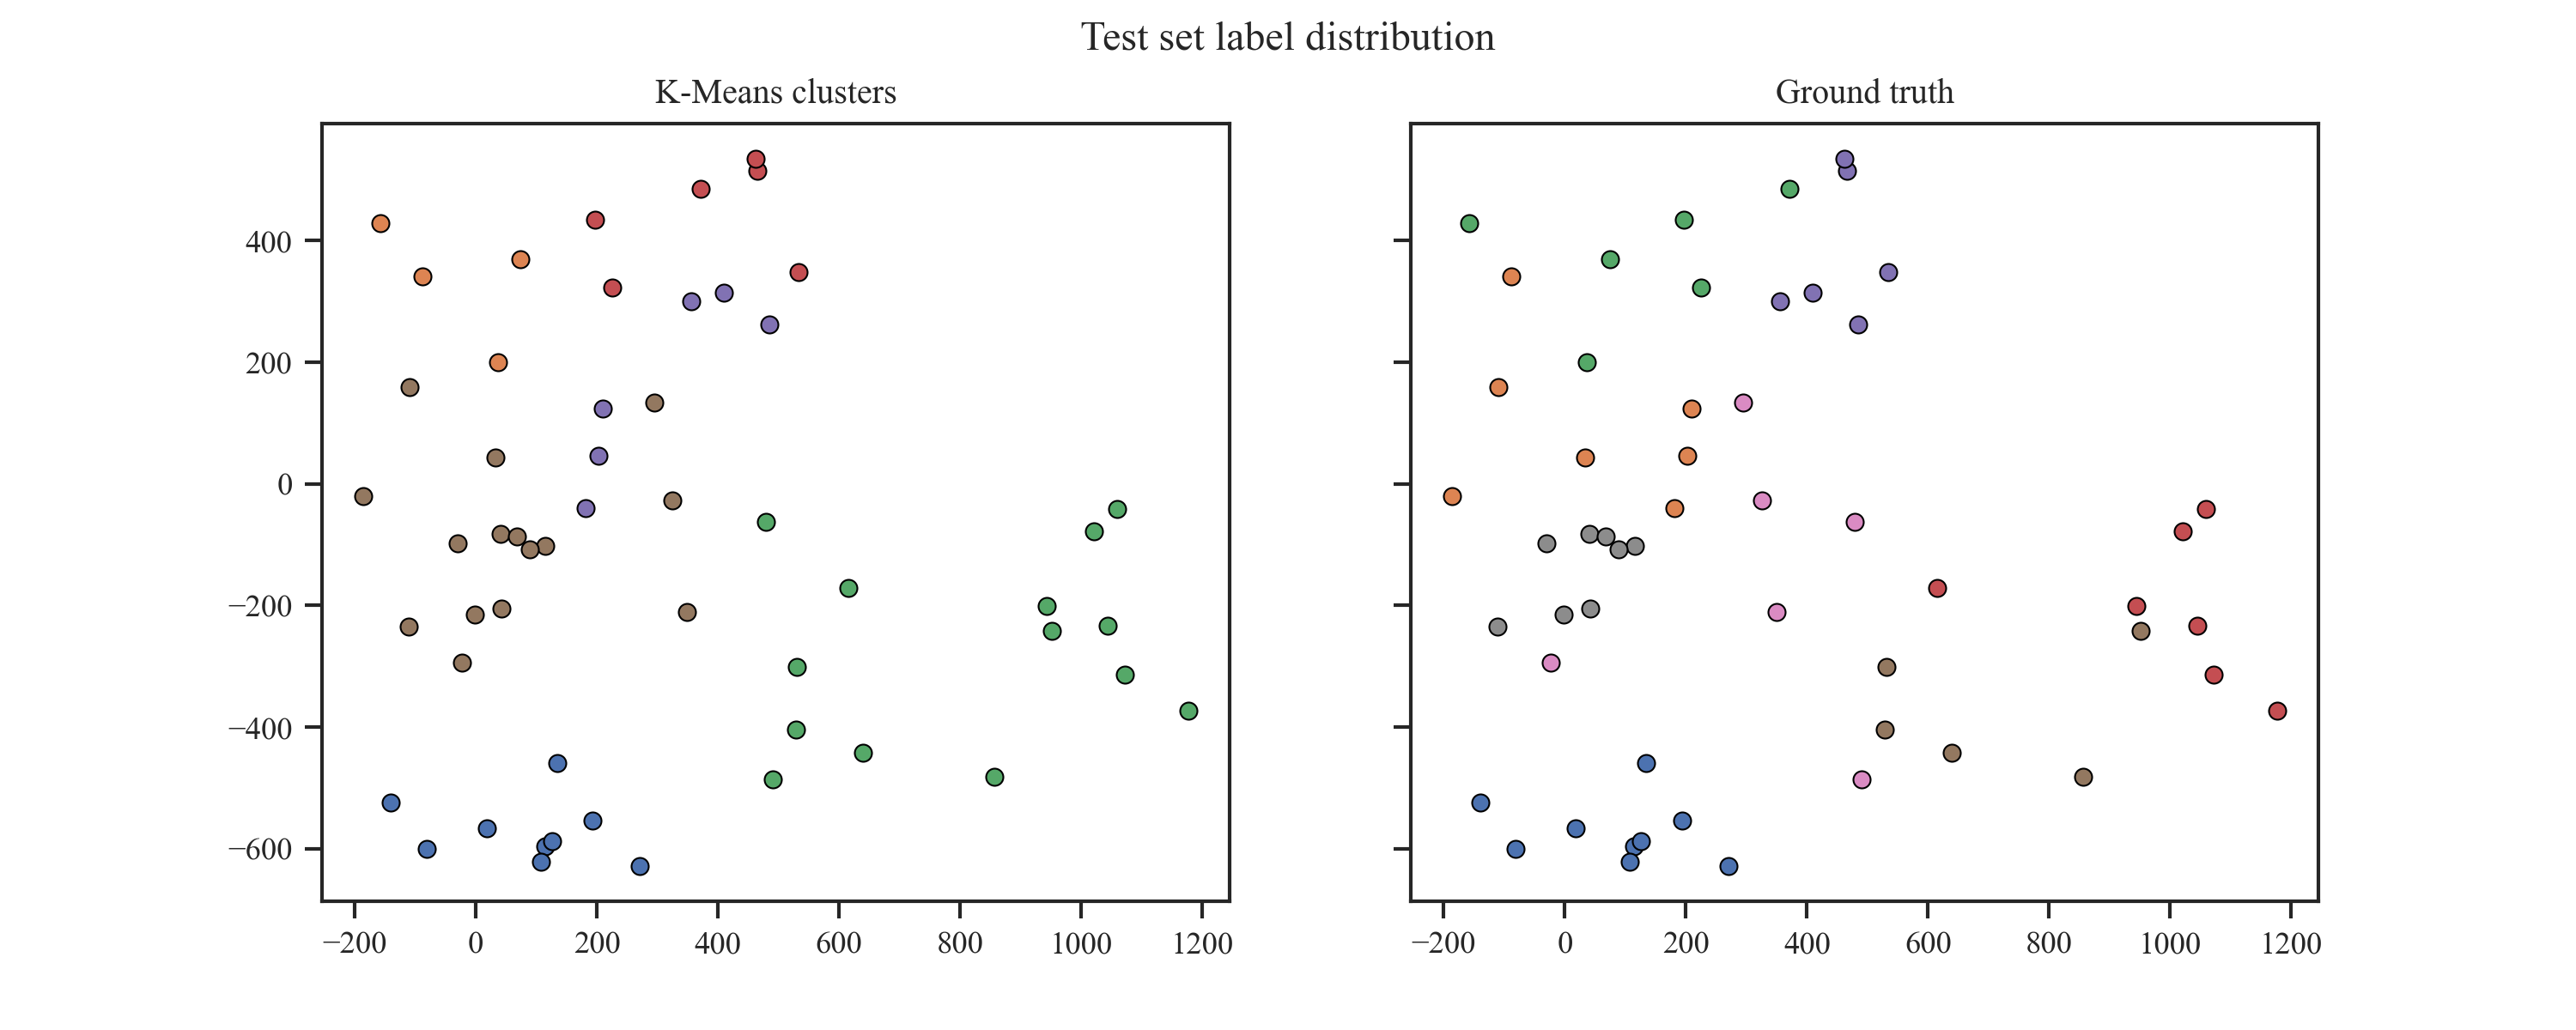
\includegraphics[width=0.7\textwidth]{img/k_means.png}}
    \caption{Comparison between K-Means clusters and ground truth labels on the speaker identification test set.}
    \label{fig:k_means}
\end{figure*}

\section{Models and Training}
\label{sec:models}

\subsection{Models}

We compared three different neural network models, which we describe below. The block diagram of the systems is illustrated in Figure~\ref{fig:block_diagram}.

\begin{figure*}[htbp]
    \centerline{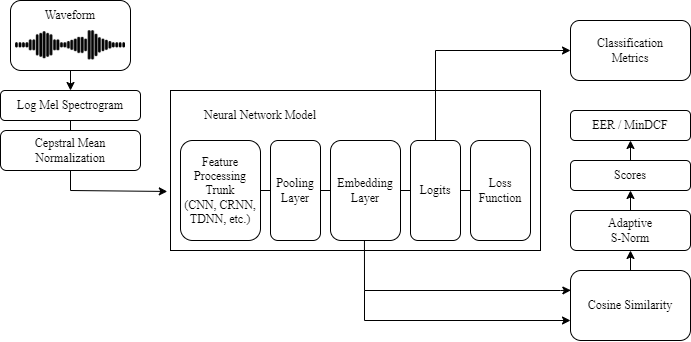
\includegraphics[width=0.7\textwidth]{img/apr_block_diagram.png}}
    \caption{Block diagram of a generic speaker recognition system.}
    \label{fig:block_diagram}
\end{figure*}

\paragraph{ResNet34-SE}

The first model is based on the ResNet34 architecture~\cite{he2016resnet}, modified to accept log Mel spectrograms as input. Following the approach described in~\cite{heo2020clova,chung2020defence}, we halved the number of channels in the convolutional layers, removed the max pooling layer, reduced the kernel size of the first convolutional layer and adopted SAP to aggregate features in the time domain. Additionally, we introduced Squeeze-and-Excitation (SE) layers~\cite{jie2020squeeze}, which proved to be good for speaker verification according to~\cite{zhang2021beijing}. For the loss function, we used SC AAM Softmax.

\paragraph{LAS-MHA}

Taking inspiration from the Listen, Attend and Spell (LAS)~\cite{irie2019las} model for sequence-to-sequence speech recognition and from the Multi-Head Attention (MHA)~\cite{vaswani2017attention} employed in language modeling, we devised a new architecture. We stacked a MHA layer with 8 heads on top of the encoder part of the LAS model, composed of CNN layers followed by bidirectional LSTM layers. A TAP layer was inserted between the CNN and LSTM layers. We used SC AAM Softmax during training.

\paragraph{EfficientNetV2}

Many state-of-the-art architectures in speaker recognition have been borrowed from the computer vision domain. For this reason, we decided to use EfficientNetV2~\cite{tan2021efficientnetv2}, a recently developed model that performs well in image classification while being optimized for training speed and parameter efficiency. EfficientNetV2 is characterized by its use of depthwise convolution in place of traditional convolution, which reduces the number of parameters. We used a simple TAP layer. EfficientNetV2 was trained with standard Softmax loss.

\subsection{Training and Scoring}

Training was carried out in two steps, according to the Large Margin Fine-Tuning strategy~\cite{thienpondt2021voxsrc}. We first trained the models on random crops of the utterances with a length of 2 seconds (eventually padded), to avoid overfitting. When the models stopped learning, we fine-tuned them with random crops of 4 seconds. We also increased the margin $m$ of SC AAM Softmax from 0.1 to 0.15 and the scale $s$ from 15 to 20. Increasing the margin makes training harder, but leads to more discriminative embeddings. Additionally, we dropped SpecAugment online data augmentation. The models were evaluated against 4 seconds random crops for identification and full length utterances for verification.

We used 256 dimensional embeddings, which were found to be the best for identification in~\cite{hajibabaei2018unified}. Adam was chosen as optimizer, with a learning rate of 0.001. 

For speaker verification, we compared the embeddings by cosine similarity and then normalized the scores with AS-Norm, using cohorts of size 100.

\section{Results}
\label{sec:results}

Considering the fact that we used a subset of VoxCeleb1 for both training and test set, a direct comparison with models described in literature is not possible. Besides, researchers often trained their models on the much larger VoxCeleb2 dataset before evaluating them on the VoxCeleb1 test set. For this reason, we added the kind of training set to the results shown in Table~\ref{tab:results}. As a baseline, we used a Support Vector Machine (SVM) with RBF kernel and parameter C equal to 1, trained on the same subset as K-Means (see Section~\ref{sec:dataset}).

Our models performed better than the baseline, but could not match the current state-of-the-art systems. We argue that literature models (i) were trained on larger datasets, which provide more diversity and variation and thus better generalization, as the models trained on VoxCeleb2 suggest; (ii) were usually trained on 6 seconds long utterances, which was not possible for us; (iii) were aggregated in fusion or ensemble systems with up to 14 models~\cite{zhang2021beijing}.

ResNet34-SE and EfficientNetV2 achieved similar performances on the identification task, but the former was clearly superior on the verification task. This can be ascribed to the more discriminative embeddings obtained with SC AAM Softmax. 

% For literature models, we reported the verification results on the original (O) verification split.

\begin{table*}[htbp]
    \caption{VoxCeleb1 Test Set Results}
    \begin{center}
        \begin{tabular}{|c|c|c|c|c|c|c|c|}
        \hline
        \textbf{Model} & \textbf{Year} & \textbf{Training Set} &  \textbf{Top1 Accuracy} & \textbf{Top5 Accuracy} & \textbf{F1 Score} & \textbf{EER(\%)} & \textbf{MinDCF}$^{\mathrm{a}}$\\
        \hline
        Nagrani et al.~\cite{nagrani2017voxceleb} & 2017 & VoxCeleb1 & 80.50 & 92.10 & - & - & - \\
        Nagrani et al.~\cite{nagrani2017voxceleb} & 2017 & VoxCeleb1 & - & - & - & 7.80 & 0.710 (0.01) \\
        Cai et al.~\cite{cai2018exploring} & 2018 & VoxCeleb1 & 89.90 & 95.70 & - & - & - \\
        Cai et al.~\cite{cai2018exploring} & 2018 & VoxCeleb1 & - & - & - & 5.27 & 0.439 \\
        Cai et al.~\cite{cai2018exploring} & 2018 & VoxCeleb1 & - & - & - & 4.46 & 0.577 \\
        % Chung et al.~\cite{chung2018voxceleb2} & 2018 & VoxCeleb1 & - & - & - & 7.8 & 0.71 (0.01) \\
        % Chung et al.~\cite{chung2018voxceleb2} & 2018 & VoxCeleb2 & - & - & - & 3.95 & 0.429 (0.01) \\
        Okabe et al.~\cite{okabe2018asp} & 2018 & VoxCeleb1 & - & - & - & 3.85 & 0.406 (0.01) \\
        Hajibabaei, Dai~\cite{hajibabaei2018unified} & 2018 & VoxCeleb1 & \textbf{94.60} & \textbf{98.10} & - & 4.69 & 0.453 (0.01) \\
        Hajibabaei, Dai~\cite{hajibabaei2018unified} & 2018 & VoxCeleb1 & 92.80 & 97.50 & - & 4.30 & 0.413 (0.01) \\
        % Snyder et al.~\cite{snyder2018xvectors}$^{\mathrm{b}}$ & 2018 & VoxCeleb2 & - & - & - & 3.10 & 0.33 (0.01) \\
        % India et al.~\cite{india2019selfmha} & 2019 & VoxCeleb1 & - & - & - & 4.0 & 0.0045 (0.01) \\
        % Xie et al.~\cite{xie2019utterance} & 2019 & VoxCeleb2 & - & - & - & 3.22 & - \\
        Chung et al.~\cite{chung2019delving} & 2019 & VoxCeleb1 & 89.00 & 96.15 & - & 5.37 & - \\
        Chung et al.~\cite{chung2019delving} & 2019 & VoxCeleb1 & 89.00 & 95.94 & - & 5.26 & - \\
        % Chung et al.~\cite{chung2020defence} & 2020 & VoxCeleb2 & - & - & - & 2.21 & - \\
        % Heo et al.~\cite{heo2020clova} & 2020 & VoxCeleb2 & - & - & - & 1.18 & 0.086 (0.05) \\
        % Desplanques et al.~\cite{desplanques2020ecapa} & 2020 & VoxCeleb2 & - & - & - & 0.87 & 0.1066 (0.01) \\
        % Nagrani et al.~\cite{nagrani2020voxceleb} & 2020 & VoxCeleb2 & - & - & - & 2.87 & 0.31 (0.01) \\
        % Xiang~\cite{xiang2020xx205} & 2020 & VoxCeleb2 & - & - & - & 0.7712 & 0.0774 (0.01) \\
        % Xiang~\cite{xiang2020xx205} & 2020 & VoxCeleb2 & - & - & - & 0.8350 & 0.0638 (0.01) \\
        Hajavi, Etemad~\cite{hajavi2021siamese} & 2021 & VoxCeleb1 & - & - & - & 3.14 & - \\
        % Kwon et al.~\cite{kwon2021ins} & 2021 & VoxCeleb2 & - & - & - & 0.73 & 0.056 (0.05)\\
        % Kwon et al.~\cite{kwon2021ins} & 2021 & VoxCeleb2 & - & - & - & 0.74 & 0.061 (0.05)\\
        % India et al.~\cite{india2021double} & 2021 & VoxCeleb2 & - & - & - & 3.19 & 0.0027 (0.01) \\
        Thienpondt et al.~\cite{thienpondt2021voxsrc} & 2021 & VoxCeleb2 & - & - & - & 0.64 & 0.070 (0.01) \\
        Thienpondt et al.~\cite{thienpondt2021voxsrc} & 2021 & VoxCeleb2 & - & - & - & 0.56 & 0.074 (0.01) \\
        Zhao et al.~\cite{zhao2021speakin} & 2021 & VoxCeleb2 & - & - & - & \textbf{0.52} & 0.050 (0.01) \\
        Zhao et al.~\cite{zhao2021speakin} & 2021 & VoxCeleb2 & - & - & - & 0.56 & \textbf{0.048 (0.01)} \\
        \hline
        \textbf{SVM (our baseline)} & 2022 & VoxCeleb1 Subset & 13.98 & - & 11.46 & - & - \\
        \textbf{ResNet34-SE (ours)} & 2022 & VoxCeleb1 Subset & 64.21 & 84.21 & 59.28 & 14.50 & 0.893 (0.01) \\
        \textbf{LAS-MHA (ours)} & 2022 & VoxCeleb1 Subset & 49.32 & 65.26 & 45.40 & 24.47 & 0.984 (0.01) \\
        \textbf{EfficientNetV2 (ours)} & 2022 & VoxCeleb1 Subset & 67.67 & 85.11 & \textbf{64.26} & 16.44 & 0.974 (0.01) \\
        \hline
        \multicolumn{8}{l}{$^{\mathrm{a}}$If provided by the Authors, we noted the $P_{\text{target}}$ value within parentheses.} \\
        % \multicolumn{8}{l}{$^{\mathrm{b}}$Results reported in~\cite{nagrani2020voxceleb}.}
        \end{tabular}
        \label{tab:results}
    \end{center}
\end{table*}
% Others, trained on VoxCeleb2: Large Margin Softmax Loss for Speaker Verification; SpeakIn Team for the VoxCeleb Speaker Recognition Challange 2020; The DKU-DukeECE Systems for VoxCeleb Speaker Recognition Challenge 2020

\section{Conclusions}
\label{sec:conclusions}

This work investigated the field of speaker recognition, illustrating the most popular techniques and comparing different neural network models. Our models, albeit far from the state-of-the-art, showed promising results, which could be improved in future research by way of larger datasets and more computational power.

\bibliographystyle{IEEEtran}
\bibliography{bibtex_entries}

\end{document}
